% Source: http://tex.stackexchange.com/a/150903/23931
\makeatletter
\def\input@path{{../}}
\makeatother
\documentclass[11pt]{article}
\usepackage[letterpaper,margin=1in]{geometry}
\usepackage{xcolor}
\usepackage{fancyhdr}
\usepackage{hyperref}
\renewcommand{\headrulewidth}{1.5pt}
\usepackage{times}
\usepackage{titlesec}
\usepackage{amsmath}
\usepackage{amssymb}
\usepackage{algorithm}
\usepackage{algorithmic}
\titlespacing*{\section}
{0pt}{0.5ex}{0.7ex}
\usepackage{lastpage}
\usepackage{color}
\usepackage{graphicx}
\usepackage{caption}

\pagestyle{fancy}
\fancyhf{}
\fancyhead[C]{%
  \footnotesize
  \fontsize{12}{12}
  \large \soptitle\hspace{1cm}
  \institution \hspace{1.2cm}
  \yourname
  }
\fancyfoot[C]{\thepage}

\newcommand{\institution}{RF excitation profile correction}
\newcommand{\soptitle}{Looping Star Development}
\newcommand{\yourname}{David Frey}
%\newcommand{\yourweb}{https://www.abcd.com/}
%\newcommand{\youremail}{email@address.edu}

\newcommand{\statement}[1]{\par\medskip
  \underline{\textcolor{blue}{\textbf{#1:}}}\space
}

\begin{document}

\section*{Motivation}
I hypothesize that one way to improve the SNR in looping star images would be to increase the flip angle of each RF subpulse.
However, because the gradients at each RF pulse is fixed, and the B1 amplitude is limited by the scanner,
the only practical way to increase the flip angle would be to increase the duration of the RF pulse.
Increasing the duration of the RF pulse will also introduce a changing excitation profile across each spoke.
Longer RF pulses will have smaller bandwidth, which will introduce a blurring effect around the edges of the image.
Higher gradient amplitudes which are required for high spatial resolution will also introduce this effect.
I propose to correct for this blurring effect by considering the excitation profile in the forward model of our reconstruction,
similar to the methods presented in \cite{Li2014}.

\section*{Mathematical representation of forward model}
A simplified forward model of the MRI signal for a single frame can be written as:
\begin{equation}\label{eq:basic_fwd}
  k = Fx
\end{equation}
where $k \in \mathbb{C}^{SM}$ is the acquired k-space data, $F \in \mathbb{C}^{SM \times N}$ is the Fourier transform matrix,
and $x \in \mathbb{C}^{N}$ is the image to be reconstructed.
For looping star data, the kspace data is acquired in a spoke-wise fashion, where $S$ is the number of spokes and $M$ the number of k-space points per spoke,
so the problem can be broken down into smaller blocks:
\begin{equation}\label{eq:spokewise_fwd}
  \begin{aligned}
    k_{i} = F_{i} x, \quad i = 1, 2, \ldots, S \\
    \rightarrow \begin{bmatrix} k_1 \\ k_2 \\ \vdots \\ k_S \end{bmatrix}
     = \begin{bmatrix} F_{1} \\ F_{2} \\ \vdots \\ F_{S} \end{bmatrix} x
  \end{aligned}
\end{equation}
where $k_{i} \in \mathbb{C}^{M}$ is the acquired k-space data for the $i$-th spoke, and $F_{i} \in \mathbb{C}^{M \times N}$ is the Fourier transform matrix for the $i$-th spoke.
Note that the number of spokes not only includes the number of excitations in one looping star shot, but also all of its projections in 3D kspace.
The excitation profile of each hard RF pulse is easily calculated using small-tip approximation:
\begin{equation}
    B1_i = \text{sinc} (\gamma \tau g_{x_i}c_x + g_{y_i}c_y + g_{z_i}c_z), \quad i = 1, 2, \ldots, S
\end{equation}
Here, $\gamma$ is the gyromagnetic ratio of hydrogen, $\tau$ is the duration of the RF pulse.
$c_x, c_y, c_z \in \mathbb{R}^N$ represent image spatial coordinates corresponding to each voxel.
$g_{x_i}, g_{y_i}, g_{z_i}$ are the gradients at the $i$-th RF pulse.
Then, the excitation profile can be included in the forward model at each spoke:
\begin{equation}\label{eq:expro_fwd}
  \begin{aligned}
    k_{i} = F_{i} \text{diag}(B1_i) x, \quad i = 1, 2, \ldots, S \\
    \rightarrow \begin{bmatrix} k_1 \\ k_2 \\ \vdots \\ k_S \end{bmatrix}
    = \begin{bmatrix} F_{1} & 0 & \cdots & 0 \\ 0 & F_{2} & \cdots & 0 \\ \vdots & \vdots & \ddots & \vdots \\ 0 & 0 & \cdots & F_{S} \end{bmatrix}
      \begin{bmatrix} \text{diag}(B1_1) \\ \text{diag}(B1_2) \\ \vdots \\ \text{diag}(B1_S) \end{bmatrix} x
  \end{aligned}
\end{equation}

\section*{Implementation}
Currently, I am implementing the reconstruction in MATLAB MIRT just to keep everything in one place with the PulSeq code,
but will try Julia too if I feel it will help fix some of the issues I'm having.

\subsection*{Nominal problem size}
For a single volume looping star acquisition, a nominal problem size could be:
\begin{itemize}
  \item $S = 736$ spokes (23 excitations, 32 projections)
  \item $M = 280$ k-space points per spoke
  \item $N \approx 2\cdot10^6$ voxels ($128 \times 128 \times 128$) image size
\end{itemize}

\subsection*{Storing excitation profiles}
Storing every excitation in a single excitation profile operator as shown in Eq.~\ref{eq:expro_fwd} would require storing
a $SN \times N$ matrix containing the profiles, which is infeasible even when using fatrix storage formats for the nominal problem size.
To get around this, I store only the rf excitation gradients and calculate the exciation profiles at each spoke during the forward operation.
\begin{algorithm}[H]
  \caption{Forward operation with excitation profile}
  \begin{algorithmic}
    \STATE $x \leftarrow \text{reshape}(x, N)$
    \FOR{$i = 1$ to $S$}
      \STATE $B1_i \leftarrow \text{sinc} (\gamma \tau g_{x_i}c_x + g_{y_i}c_y + g_{z_i}c_z)$
      \STATE $k_i \leftarrow F_i \text{diag}(B1_i) x$
    \ENDFOR
    \STATE $k \leftarrow \text{reshape}([k_1, k_2, \ldots, k_S], SM)$
  \end{algorithmic}
\end{algorithm}

\subsection*{Block-wise NUFFT operations}
If $F$ were a simple DFT matrix as in cartesian imaging, I would expect the representations in Eqs.~\ref{eq:basic_fwd} and ~\ref{eq:spokewise_fwd}
to be equivalent and have similar computational cost since
the volume-wise DFT will have complexity $O(SMN)$ and the $S$ block-wise DFTs will each have complexity $O(MN)$
before considering FFT acceleration.
However, because $F$ is a NUFFT operator, I am not sure if the block-wise matrix representation still holds.
To test this, I calculated the adjoint operation for the two representations for a small dataset with only 4 projections ($S = 69$).
\begin{figure}[H]
  \centering
  \begin{minipage}{0.45\textwidth}
    \centering
    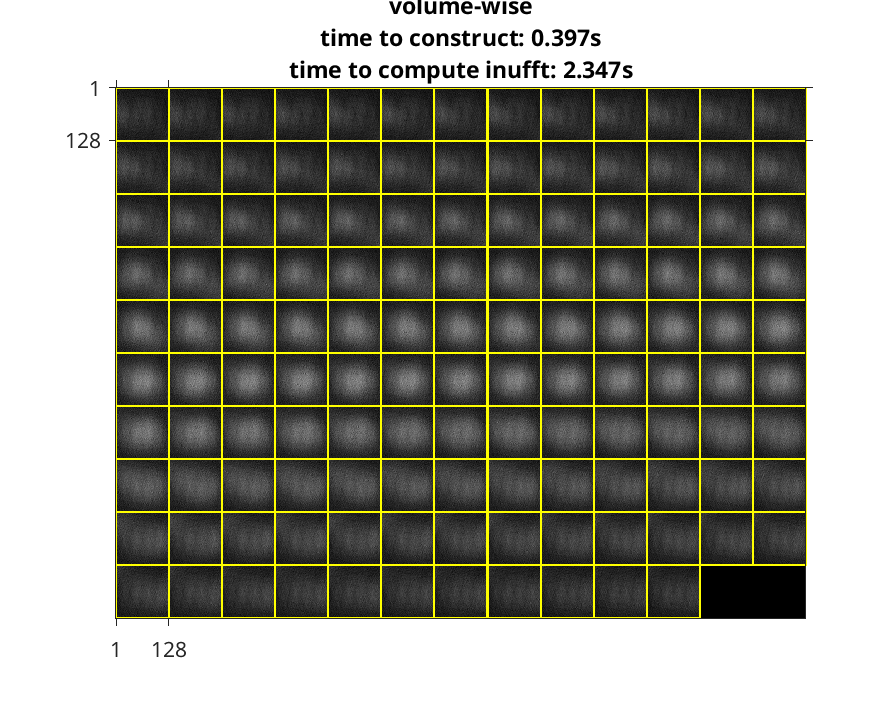
\includegraphics[width=\textwidth]{volume-wise_inufft.png}
    \caption*{(a) Volume-wise (whole) adjoint operation (iNUFFT)}
  \end{minipage}
  \hfill
  \begin{minipage}{0.45\textwidth}
    \centering
    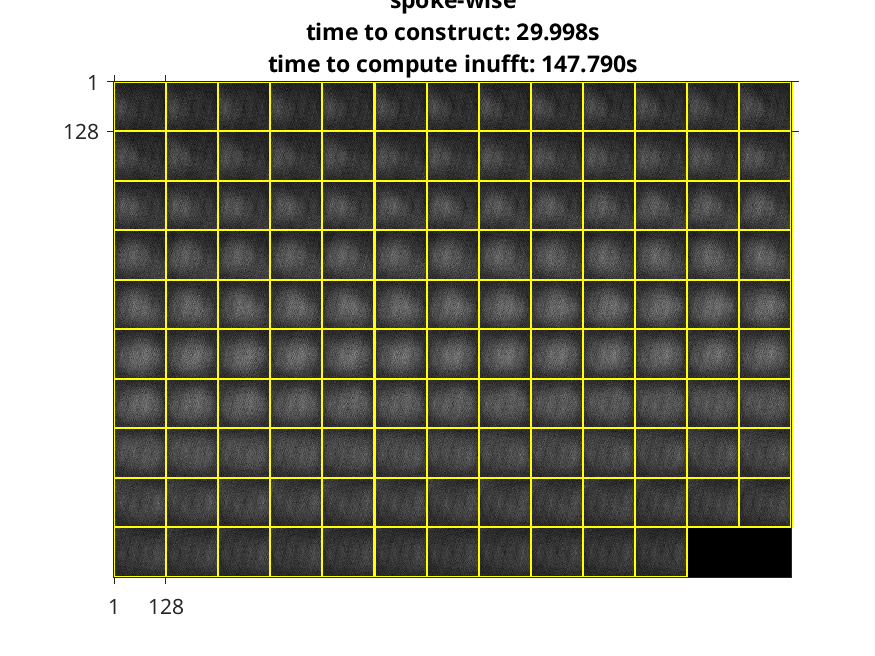
\includegraphics[width=\textwidth]{spoke-wise_inufft.png}
    \caption*{(b) Spoke-wise (block-wise) adjoint operation (iNUFFT)}
  \end{minipage}
  \caption{Comparison of adjoint operations using whole and block-wise NUFFT operators.}
  \label{fig:comparing_inuffts}
\end{figure}
As shown in figure \ref{fig:comparing_inuffts}, the adjoint operations using the whole and block-wise NUFFT operators
are not equivalent, which suggests that the block-wise representation is not valid for NUFFT operators.
Additionally, it took about $60\times$ longer to calculate the adjoint operation using the block-wise representation.
This is not an acceptable performance hit for the nominal problem size, so I will need to find a way to use the volume-wise NUFFT operator.

\bibliographystyle{plain}
\bibliography{refs}

\end{document}